%!TEX TS-program = xelatex
\documentclass[]{friggeri-cv}
\usepackage{afterpage}
\usepackage{hyperref}
\usepackage{color}
\usepackage{xcolor}
\hypersetup{
    pdftitle={},
    pdfauthor={},
    pdfsubject={},
    pdfkeywords={},
    colorlinks=false,       % no lik border color
   allbordercolors=white    % white border color for all
}
\addbibresource{bibliography.bib}
\RequirePackage{xcolor}
\definecolor{pblue}{HTML}{0395DE}

\begin{document}
\header{Dr Clément}{Thorey}
      {Data scientist}
      
% Fake text to add separator      
\fcolorbox{white}{gray}{\parbox{\dimexpr\textwidth-2\fboxsep-2\fboxrule}{%
.....
}}


% In the aside, each new line forces a line break
\begin{aside}
  \section{Address}
    Rue du Mont Cenis, 125
    75018, Paris, France
    ~
  \section{Tel \& Skype}
    +33 695 764 726
    thorey.clement
    ~
  \section{Mail}
    \href{mailto:clement.thorey@gmail.com}{\textbf{clement.thorey@}\\gmail.com}
    ~
  \section{Web \& Git}
    \href{https://github.com/cthorey}{github.com/cthorey}
    \href{http://cthorey.github.io./}{cthorey.github.io}
    \href{https://scholar.google.fr/citations?user=p5M6SxAAAAAJ&hl=fr&oi=ao}{scholar.google.fr/thorey}
    \href{https://www.kaggle.com/cthorey/}{kaggle.com/cthorey}
    ~
  \section{Python library}
    \href{http://pdsimage.readthedocs.org/en/latest/}{pdsimage}
  ~  
  \section{Programming}
    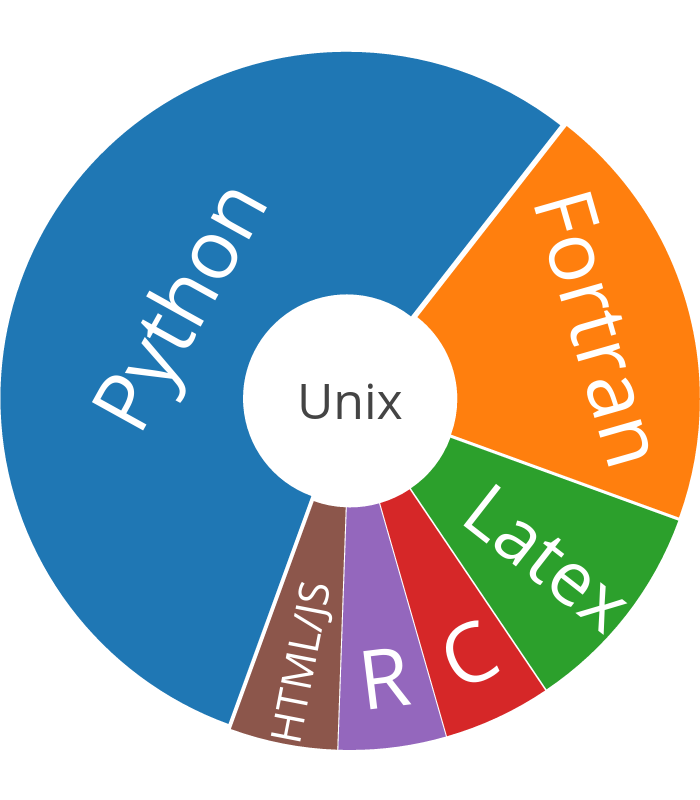
\includegraphics[scale=0.15]{img/programing.png}
    ~
  \section{PhD skills}
    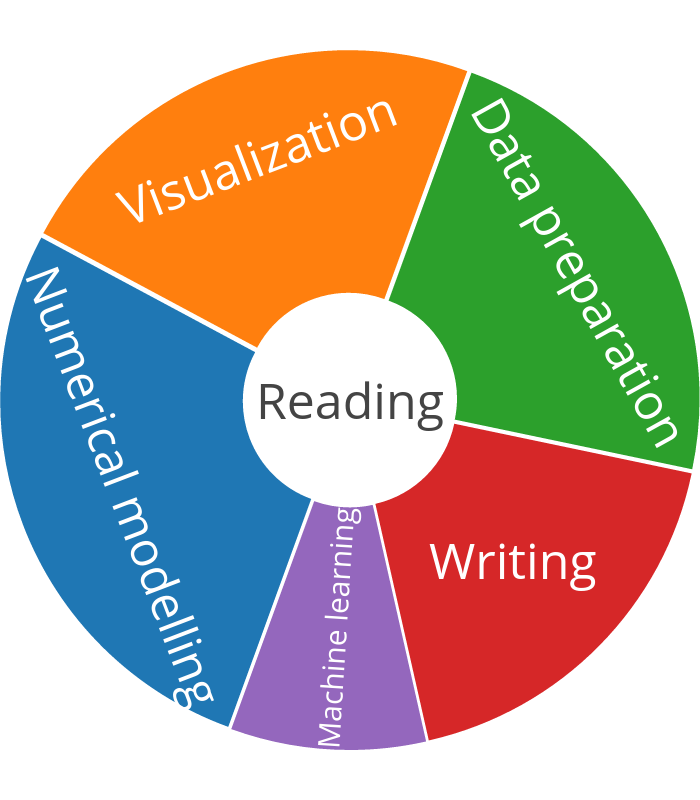
\includegraphics[scale=0.15]{img/PhD.png}
    ~
\end{aside}

\section{Research Experience}
\begin{entrylist}
  \entry  {12/10 -  15/11}  {PhD in  Geophysics (Planetary  Sciences)}
  {\href{http://www.ipgp.fr/fr/pss/planetologie-sciences-spatiales}{Institut
      de Physique du Globe, France.}}
  {Topic: Intrusive magmatism on terrestrial planets. \\
    Methods : Numerical simulation /  Data analysis. \\} \entry {11/11
    - 11/07} {Research assistant} {\href{http://ciiv.ucol.mx/}{Faculty
      of Science, University of Colima, Mexico.}}
  {Topic: Active volcano monitoring. \\
    Methods:  Seismic  activity,  thermal  imaging,  CO2  release  and
    deformation  mapping (GPS).  Data  preprocessing and  analysis.\\}
  \entry      {10/05      -      10/08}      {Research      assistant}
  {\href{http://lisgi1.engr.ccny.cuny.edu/}{Benjamin Levich Institut},
    New York,  USA.}  {Topic :  Investigation of the  periodic jamming
    and unjamming of dense suspensions
    in a particular geometry.\\
    Methods :Experiments, Particle tracking (PIV).\\}
\end{entrylist}


\section{Teaching}
\begin{entrylist}
  \entry
    {12/10 - Now}
    {Teaching assistant}
    {Université Paris Diderot - Paris, France.}
    {Mathematics - Linear algebra, ODP, EDP, Fourrier series, Fourrier transform
    Physics - Mechanics, Experimental Physics (undergraduate level)\\
    Informatics - C (graduate level), Python (undergraduate level).\\}
\end{entrylist}

\section{Education}
\begin{entrylist}
  \entry
  {2012 - 2015}
  {PhD in Geophysics (Planetary Sciences)}
  {Institut de Physique du Globe, Paris.}
  {Thesis title: Dynamics of shallow magmatic intrusions\\
    Advisor: Chloé Michaut and Mark Wieczorek\\
    Mention: Highest distinction.}
  \entry
  {2011 - 2012}
  {Master's Degree in Earth Science}
  {Institut de Physique du Globe, Paris, France.}
  {Main subjects: Volcanology, Seismology, Geophysical Fluid Dynamics.\\
    Mention: Honors. \\}
  \entry
  {2009 - 2011}
  {Master's Degree in Theoretical Physics and Chemistry}
  {ENS Lyon, France.}
  {Main subjects: Entire spectrum of physics and chemistry.\\
    Mention: Honors.\\}
  \entry
  {2008 - 2009}
  {Bachelor's Degree in Physics and Chemistry.}
  {ENS Lyon, France.}
  {Main subjects: Physics and chemistry such as quantum physics and statistical physics.  Mathematics and computer science. \emph{ENS is a French elite graduate school recruiting among the top 1\% of science students}.\\}
  \entry
  {2006-2008}
  {Bachelor's Degree MPSI.}
  {Université Lille 1, Lille, France.}
  {Main subjects : Mathematics, Physics and Computer Science\\
    Mention: Honors.}
\end{entrylist}

\newpage

\begin{aside}
~
~
~
  \section{Personal Skills}
    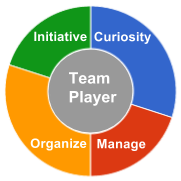
\includegraphics[scale=0.62]{img/personal.png}
    ~
  \section{Homes/Confs}
    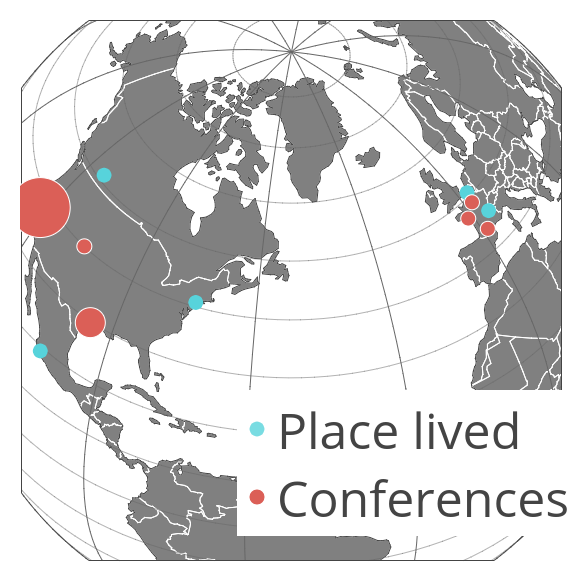
\includegraphics[scale=0.2]{img/map.png}
    ~
  \section{Languages}
    \textbf{French}
\includegraphics[scale=0.40]{img/5stars.png}
    \textbf{English}
\includegraphics[scale=0.40]{img/4stars.png}
    \textbf{Spanish}
\includegraphics[scale=0.40]{img/4stars.png}
\end{aside}

\section{Complementary education: Formation/MOC}
\begin{itemize}
\item \textbf{High performance computing training} \\
Course instructor: Cédric Castagnède (ClusterVision)\\
Topic: GPU programming (CUDA).

\item            \href{http://www.cs.cmu.edu/~tom/10701_sp11/}{\textbf{Machine
    learning}}\\
 Course instructor: Tom Mitchell - Carnegie Mellon University\\
    Topics : Bayesian networks,  decision tree learning, Support Vector
    Machines, statistical learning  methods, unsupervised learning and
    reinforcement learning.
\item   \href{http://cs231n.github.io/}{\textbf{Convolutional   Neural
    Networks for Visual Recognition}}\\
Course instructor : Fei-Fei Li, Andrej Karpathy, Justin Johnson - Standford\\
Topics : Support Vector  Machine, Neural networks, Convolutional Neural
Networks,    Recurrent    Neural    Networks,    Long    Short    Term
Memory,Reinforcement Learning.\\
Assignments : \href{https://github.com/cthorey/CS231}{cthorey/CS231}
\item
  \href{http://camdavidsonpilon.github.io/Probabilistic-Programming-and-Bayesian-Methods-for-Hackers/}{\textbf{Probabilistic
    Programming and Bayesian Methods for Hackers}}\\
Topic : Bayesian modeling.
\end{itemize}


\section{Peer-Reviewed Articles}
\begin{itemize}
\item \textbf{Thorey, C.}, Michaut,  C., 2015.  Elastic-plated gravity
  current  with  temperature-dependent  viscosity.  Journal  of  Fluid
  Mechaniscs 
\item  \textbf{Thorey,  C.},  Michaut,   C.,  Wieczorek,  M.A.,  2015.
  Gravitational  signatures of  lunar floor-fractured  craters.  Earth
  and Planetary Science Letters
  1–40. \\
  doi:10.1016/j.epsl.2015.04.021
\item \textbf{Thorey, C.}, Michaut, C., 2014. A model for the dynamics
  of crater-centered  intrusion: Application to  lunar floor-fractured
  craters.       J.       Geophys.        Res.       Planets      119,
  286–312. \\
  doi:10.1002/2013je004467
\item Michaut,  C., Baratoux, D., \textbf{Thorey,  C.}, 2013. Magmatic
  intrusions and  deglaciation at mid-latitude in  the northern plains
  of Mars. Icarus 225, 602–613. \\
  doi:10.1016/j.icarus.2013.04.015
\end{itemize}

\section{Communications in major scientific conferences}
\begin{itemize}
\item  C. Michaut  and  \textbf{Thorey, C.},  Magmatism  on the  Moon,
  European Geophysical Union conference 2016, Talk, Vienna.
\item \textbf{Thorey,  C.}, Floor-Fractured Crater  detections through
  Machine Learning  Methods, American  Geophysical Union Fall meeting
  2015, Poster, San Francisco.
\item \textbf{Thorey, C.} and C.  Michaut, A General Model for Shallow
  Magmatic Intrusion,  American Geophysical  Union Fall  meeting 2015,
  Poster, San Francisco.
\item \textbf{Thorey, C.}, Detection  of lunar floor-fractured craters
  using   machine  learning   methods,   European  Planetary   Science
  conference 2015, Poster, Nantes.
\item C. Michaut  and \textbf{Thorey, C.}, Magmatic  intrusions in the
  lunar  crust,  European  Planetary Science  conference  2015,  Talk,
  Nantes.
\item \textbf{Thorey,  C.} and  C. Michaut,  Effect of  a temperature-dependent
  viscosity on  the spreading  of laccoliths,  AGU Fall  meeting 2014,
  Poster, San Francisco.
\item \textbf{Thorey,  C.}, C.  Michaut, M.  Wieczorek, Gravitational signatures
  of lunar  floor fractured craters,  GRAIL science meeting  may 2014,
  Talk, Boulder.
\item  \textbf{Thorey, C.},  Gravitational signatures  of lunar  floor
  fractured  craters, Workshop  Structure and  Dynamics of  Earth-like
  Planets, Collège de France, Poster, November 2014, Paris.
\item \textbf{Thorey,  C.}, Les cratères au sol fracturé: Témoins
  d'un magmatisme  intrusif passé  sur la Lune.   UnivEarths, November
  2014, Talk.
\item \textbf{Thorey,  C.}, C.  Michaut, M.   Wieczorek, Gravitational
  signatures of lunar floor fractured  craters, 45th LPSC, March 2014,
  Poster, Houston.
\item  \textbf{Thorey,  C.}   and Michaut  C.,  Thermal evolution  of a  magmatic
  intrusion, AGU Fall meeting 2013, Poster, San Francisco.
\item \textbf{Thorey,  C.} and Michaut C.,  Floor-fractured craters on the Moon :
  an evidence  of past intrusive  magmatism, 44th Lunar  and Planetary
  Science Conference, March 2013, Talk, Houston.
\item \textbf{Thorey,  C.} and Michaut C.,  Floor-fractured craters on the Moon :
  an evidence  of past intrusive  magmatic activity, AGU  Fall meeting
  2012, Poster, San Francisco.
\end{itemize}
~
~

\begin{flushleft}
\emph{February 25th, 2016}
\end{flushleft}
\begin{flushright}
\emph{Clément Thorey}
\end{flushright}


\end{document}

%%% Local Variables:
%%% mode: latex
%%% TeX-master: t
%%% End:
